\chapter{Расчёт на прочность двухслойного соединения кристалл-кристаллодержатель}

\section{Техническое задание}

Дано: 
\begin{itemize}
    \item материал кристалла:
        \BPChem{Si} ($E_1 = 1.7 \cdot 10^5 \text{ МПа}$, $\sigma_{в_1} = 700 \text{ МПа}$, $\mu_1 = 0.27$);
    \item толщина кристалла:
        $h_1 = 0.30 \text{ мм}$;
    \item материал кристаллодержателя:
        \BPChem{Ni} ($E_2 = 2.23 \cdot 10^5 \text{ МПа}$, $\sigma_{в_2} = 450 \text{ МПа}$, $\mu_2 = 0.30$);
    \item толщина кристаллодержателя:
        $h_2 = 0.22 \text{ мм}$;
    \item размер сборки в плане:
        $a = 10 \text{ мм}$, $b = 12 \text{ мм}$;
    \item число интерференционных колец вдоль стороны $a$:
        $n_x = 50$;
    \item число интерференционных колец вдоль стороны $b$:
        $n_z = 72$;
    \item длина волны лазера:
        $\lambda = 630 \text{ нм} = 0.63 \cdot 10^{-3} \text{ мм}$.
\end{itemize}

\begin{figure}[h]
    \centering
    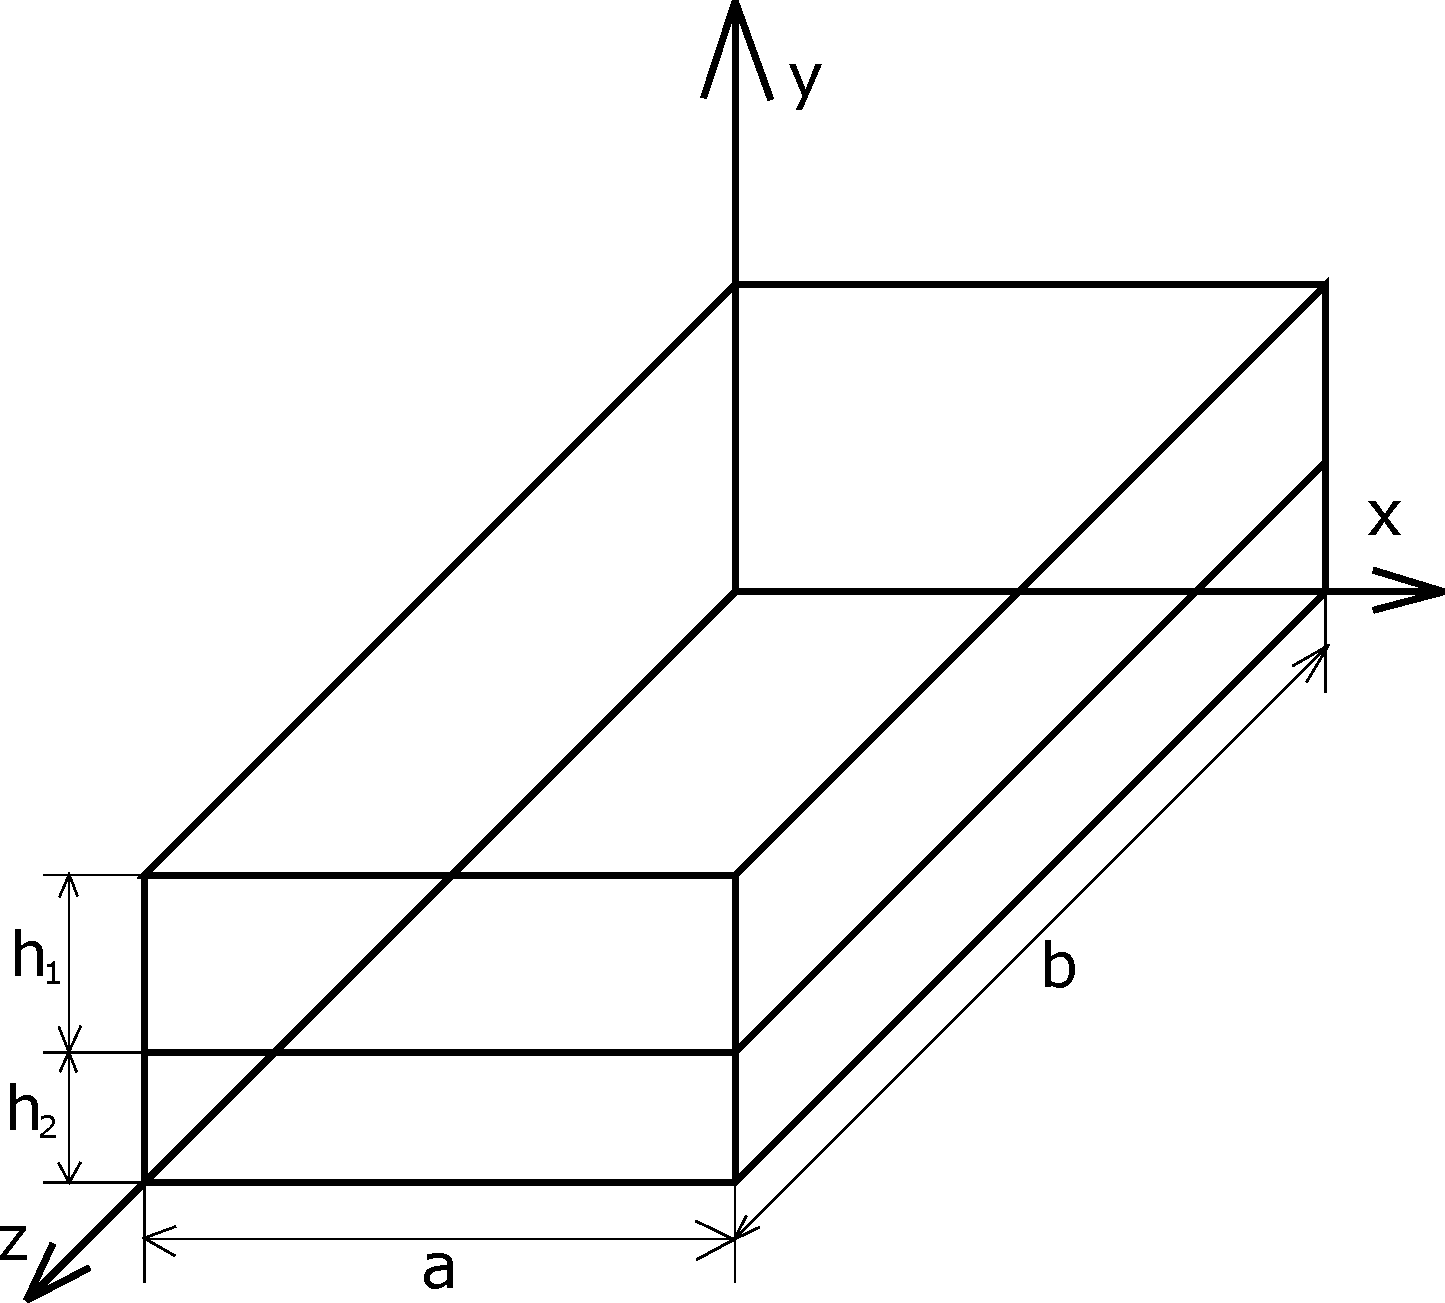
\includegraphics[width=0.5\linewidth]{assemble.pdf}
    \caption{Соединение с помощью пайки или приклейки}
\end{figure}

\begin{figure}[h]
    \centering
    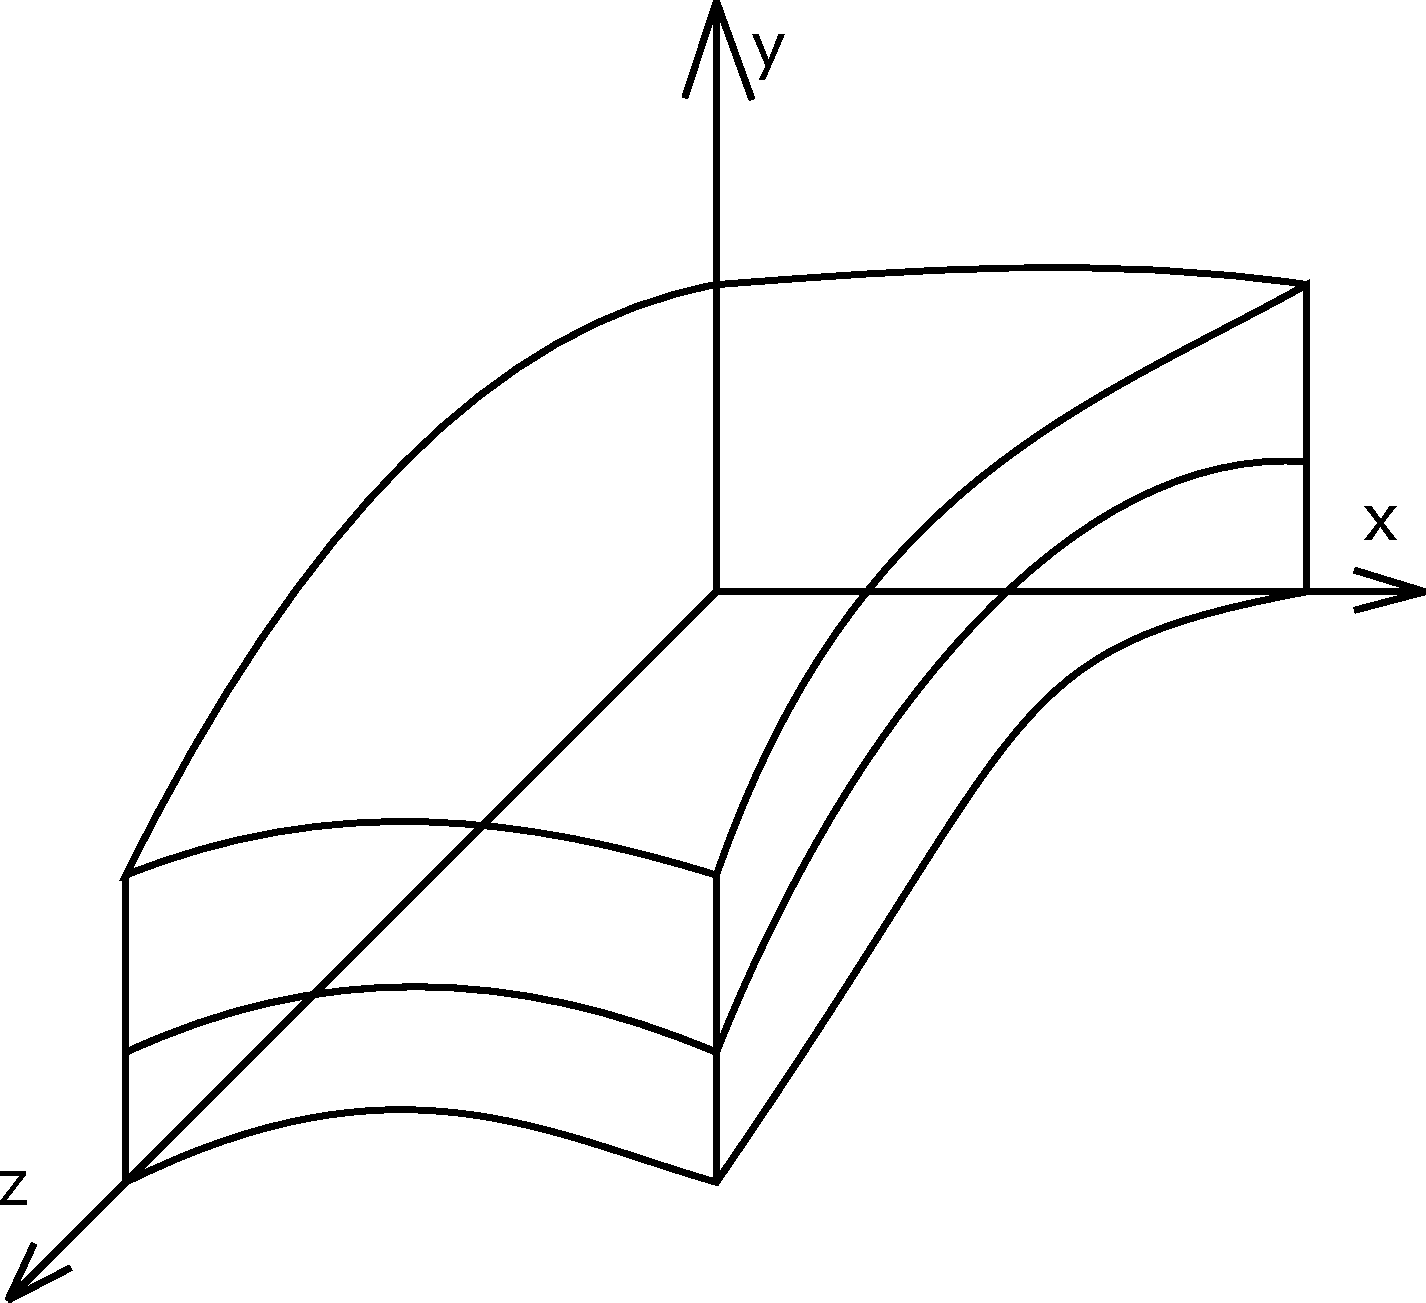
\includegraphics[width=0.5\linewidth]{flexed-assemble.pdf}
    \caption{Изгиб}
\end{figure}

\section{Решение}

1. Рассмотрим плоскость $yOx$. Определим радиус кривизны вдоль короткой стороны сборки после охлаждения, учитывая при этом, что характерный размер вдоль оси $x$ равен $D_x = a = 10 \text{ мм}$:
\[
    \rho_x = \frac{D_x^2}{4 n_x \lambda} = \frac{10^2}{4 \cdot 50 \cdot 0.63 \cdot 10^{-3}} \approx 793.7 \text{ мм}.
\]

\begin{figure}[h]
    \centering
    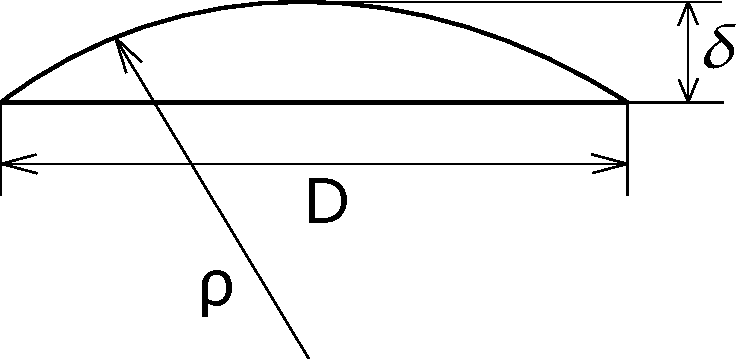
\includegraphics[width=0.4\linewidth]{flexed-unface.pdf}
    \caption{Вид изгиба в сечении}
    \label{fig:flexed-unface}
\end{figure}

Определим положение нейтрального слоя относительно границы раздела:
\[
    A = \frac{E_2 h_2^2 - E_1 h_1^2}{2 \left(E_2 h_2 + E_1 h_1\right)}
      = \frac{2.23 \cdot 10^5 \cdot 0.3^2 - 1.7 \cdot 10^5 \cdot 0.22^2}{2 \cdot (2.23 \cdot 10^5 \cdot 0.3 + 1.7 \cdot 10^5 \cdot 0.22)}
      \approx -0.0225 \text{ мм}.
\]

Т.к. $A$ отрицательное ($A < 0$), то нейтральный слой сборки расположен выше границы раздела (Рис. \ref{fig:neutral-layer}).

\begin{figure}[h]
    \centering
    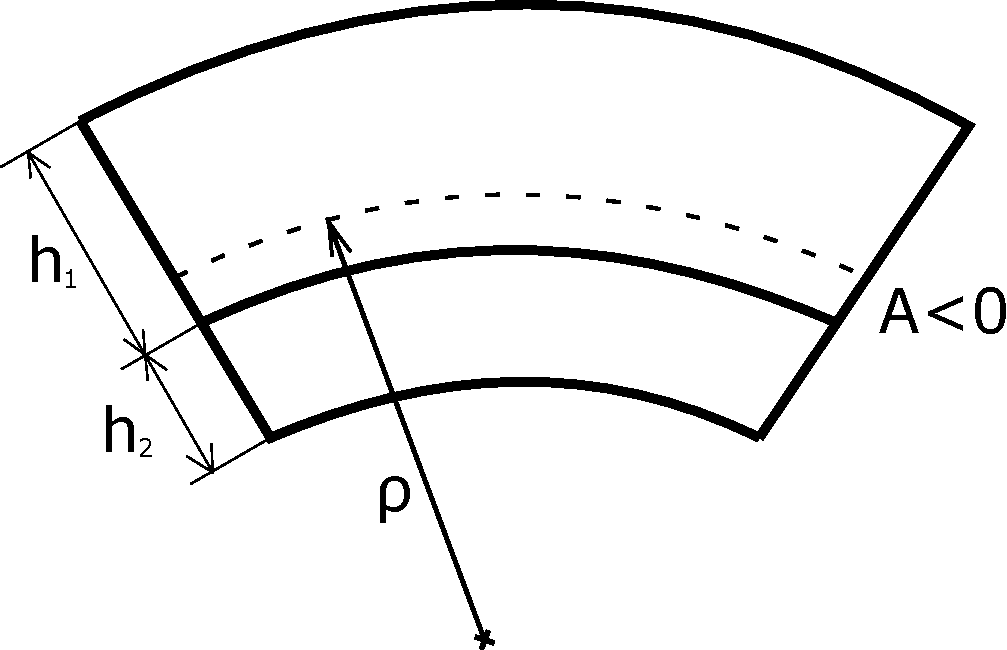
\includegraphics[width=0.3\linewidth]{neutral-layer.pdf}
    \caption{Положение нейтрального слоя}
    \label{fig:neutral-layer}
\end{figure}

Определим координаты верхней $y_{1\max}$ и нижней $y_{1\min}$ поверхностей кристалла относительно нейтрального слоя (Рис. \ref{fig:free-surface}):
\begin{equation}
    \begin{aligned}
        y_{1\max} & = A + h_1 = -0.0225 + 0.30 = 0.2775 \text{ мм}; \\
        y_{1\min} & = A = -0.0225 \text{ мм}.
    \end{aligned}
\end{equation}

Определим координаты верхней $y_{2\max}$ и нижней $y_{2\min}$ поверхностей кристаллодержателя (Рис. \ref{fig:free-surface}):
\begin{equation}
    \begin{aligned}
        y_{2\max} & = A = -0.0225 \text{ мм}; \\
        y_{2\min} & = A - h_2 = -0.0225 - 0.22 = -0.2425 \text{ мм}.
    \end{aligned}
\end{equation}

\begin{figure}[h]
    \centering
    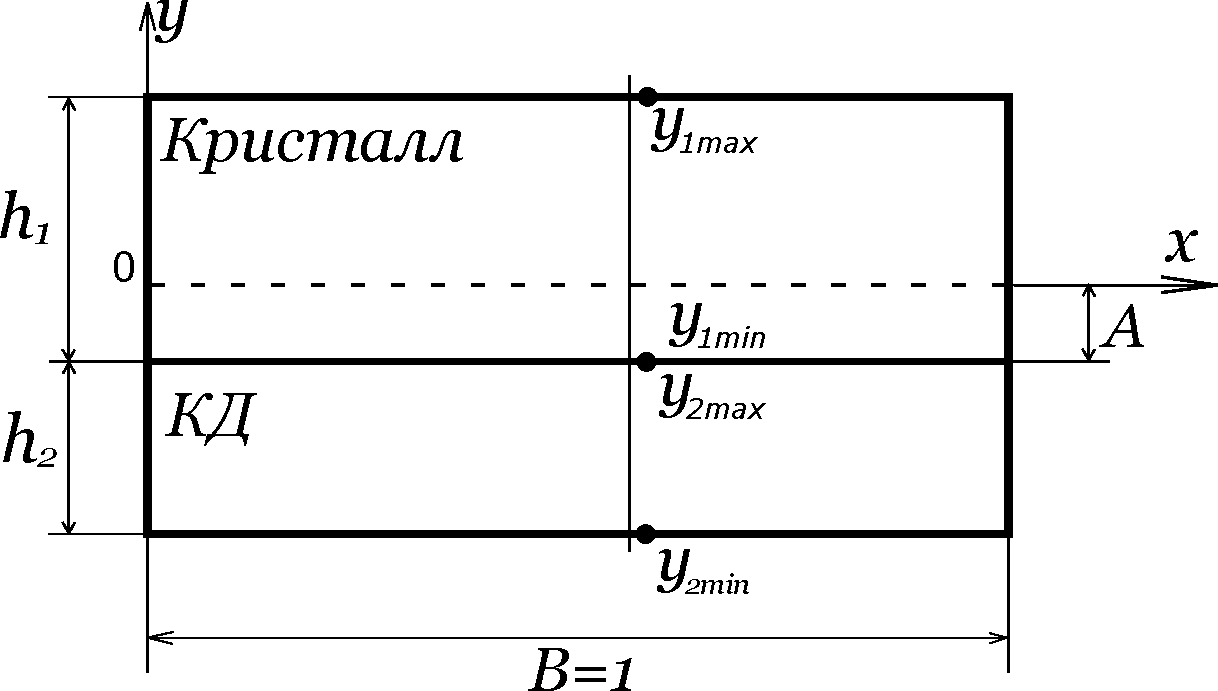
\includegraphics[width=0.5\linewidth]{free-surface.pdf}
    \caption{Расположение точек на свободных поверхностях}
    \label{fig:free-surface}
\end{figure}

Определим момент инерции кристалла единичной ширины относительно нейтрального слоя (нейтральной линии):
\[
    I_1 = \frac{(h_1 + A)^3 - A^3}{3}
        = \frac{(0.30 - 0.0225)^3 - (-0.0225)^3}{3}
        \approx 0.71 \cdot 10^{-2} \text{ } \frac{мм^4}{мм}.
\]

Определим момент инерции кристаллодержателя единичной ширины относительно нейтрального слоя (нейтральной линии):
\[
    I_2 = \frac{(h_2 - A)^3 + A^3}{3}
        = \frac{(0.22 + 0.0225)^3 + (-0.0225)^3}{3}
        \approx 0.48 \cdot 10^{-2} \text{ } \frac{мм^4}{мм}.
\]

Определим погонный момент, изгибающий пластину:
\[
    M = \frac{E_1 I_1 + E_2 I_2}{\rho_x}
      = \frac{1.7 \cdot 10^5 \cdot 0.71 \cdot 10^{-2} + 2.23 \cdot 10^5 \cdot 0.48 \cdot 10^{-2}}{793.7}
      \approx 2.86 \text{ } \frac{Н \cdot мм}{мм}.
\]

Определим нормальные силы, действующие в слоях:
\[
    N_1 = N_2 = N
        = \frac{2M}{(h_1 + h_2)}
        = \frac{2 \cdot 2.86}{0.30 + 0.22}
        \approx 11.00 \text{ } \frac{Н}{мм}.
\]

\begin{figure}[h]
    \centering
    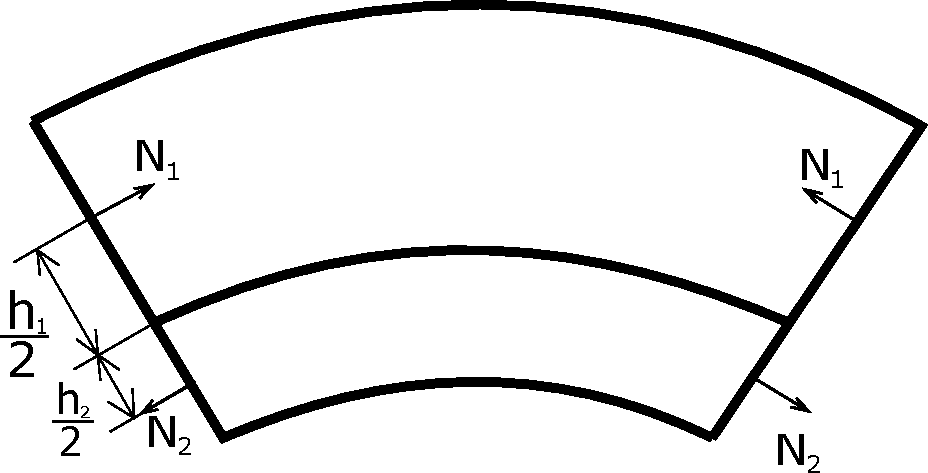
\includegraphics[width=0.3\linewidth]{normal-forces.pdf}
    \caption{Нормальные силы}
    \label{fig:normal-forces}
\end{figure}

Определим напряжение в кристалле на верхней свободной поверхности:
\[
    \sigma_{кр \max} = \frac{1}{1 - \mu_1} \left(\frac{E_1 y_{1\max}}{\rho_x} - \frac{N}{h_1}\right)
                     = \frac{1}{1 - 0.27} \left(\frac{1.7 \cdot 10^5 \cdot 0.2775}{793.7} - \frac{11.00}{0.30}\right)
                     \approx 31.2 \text{ } МПа.
\]

Определим напряжение в кристалле на на границе раздела с кристаллодержателем:
\[
    \sigma_{кр \max} = \frac{1}{1 - \mu_1} \left(\frac{E_1 y_{1\min}}{\rho_x} - \frac{N}{h_1}\right)
                     = \frac{1}{1 - 0.27} \left(\frac{1.7 \cdot 10^5 \cdot (-0.0225)}{793.7} - \frac{11.00}{0.30}\right)
                     \approx -56.9\text{ } МПа.
\]

Определим напряжение в кристаллодержателе на границе раздела с кристаллом:
\[
    \sigma_{кр \max} = \frac{1}{1 - \mu_2} \left(\frac{E_2 y_{2\max}}{\rho_x} + \frac{N}{h_2}\right)
                     = \frac{1}{1 - 0.30} \left(\frac{2.23 \cdot 10^5 \cdot (-0.0225)}{793.7} - \frac{11.00}{0.22}\right)
                     \approx 62.4\text{ } МПа.
\]

Определим напряжение в кристаллодержателе на нижней свободной поверхности:
\[
    \sigma_{кр \max} = \frac{1}{1 - \mu_1} \left(\frac{E_1 y_{1\max}}{\rho_x} + \frac{N}{h_1}\right)
                     = \frac{1}{1 - 0.30} \left(\frac{2.23 \cdot 10^5 \cdot (-0.2425)}{793.7} - \frac{11.00}{0.22}\right)
                     \approx -25.9\text{ } МПа.
\]

2. Рассмотрим плоскость $yOz$. Определим радиус кривизны вдоль длинной стороны сборки после охлаждения, учитывыя при этом, что характерный размер вдоль оси $z$ равна $D_z = b = 12 \text{ } мм$:
\[
    \rho_z = \frac{D_z^2}{4 n_z \lambda}
           = \frac{12^2}{4 \cdot 72 \cdot 0.63 \cdot 10^{-3}}
           = 793.7.
\]

Так как $\rho_z = \rho_x$, то значения $A$, $y_{1 \max}$, $y_{1 \min}$, $y_{2 \max}$, $y_{2 \min}$, $I_1$, $I_2$ те же, что и для расчёта напряжений по короткой стороне сборки.

Определим погонный момент, изгибающий пластину:
\[
    M = \frac{E_1 I_1 + E_2 I_2}{\rho_z}
      = \frac{1.7 \cdot 10^5 \cdot 0.71 \cdot 10^{-2} + 2.23 \cdot 10^5 \cdot 0.48 \cdot 10^{-2}}{793.7}
      \approx 2.86 \text{ } \frac{Н \cdot мм}{мм}.
\]

Определим нормальные силы, действующие в слоях:
\[
    N_1 = N_2 = N
        = \frac{2M}{(h_1 + h_2)}
        = \frac{2 \cdot 2.86}{0.30 + 0.22}
        \approx 11.00 \text{ } \frac{Н}{мм}.
\]

Определим напряжение в кристалле на верхней свободной поверхности:
\[
    \sigma_{кр \max} = \frac{1}{1 - \mu_1} \left(\frac{E_1 y_{1\max}}{\rho_z} - \frac{N}{h_1}\right)
                     = \frac{1}{1 - 0.27} \left(\frac{1.7 \cdot 10^5 \cdot 0.2775}{793.7} - \frac{11.00}{0.30}\right)
                     \approx 31.2 \text{ } МПа.
\]

Определим напряжение в кристалле на на границе раздела с кристаллодержателем:
\[
    \sigma_{кр \max} = \frac{1}{1 - \mu_1} \left(\frac{E_1 y_{1\min}}{\rho_z} - \frac{N}{h_1}\right)
                     = \frac{1}{1 - 0.27} \left(\frac{1.7 \cdot 10^5 \cdot (-0.0225)}{793.7} - \frac{11.00}{0.30}\right)
                     \approx -56.9\text{ } МПа.
\]

Определим напряжение в кристаллодержателе на границе раздела с кристаллом:
\[
    \sigma_{кр \max} = \frac{1}{1 - \mu_2} \left(\frac{E_2 y_{2\max}}{\rho_z} + \frac{N}{h_2}\right)
                     = \frac{1}{1 - 0.30} \left(\frac{2.23 \cdot 10^5 \cdot (-0.0225)}{793.7} - \frac{11.00}{0.22}\right)
                     \approx 62.4\text{ } МПа.
\]

Определим напряжение в кристаллодержателе на нижней свободной поверхности:
\[
    \sigma_{кр \max} = \frac{1}{1 - \mu_1} \left(\frac{E_1 y_{1\max}}{\rho_z} + \frac{N}{h_1}\right)
                     = \frac{1}{1 - 0.30} \left(\frac{2.23 \cdot 10^5 \cdot (-0.2425)}{793.7} - \frac{11.00}{0.22}\right)
                     \approx -25.9\text{ } МПа.
\]

На основании полученных результатов строим эпюры распределения нормальных напряжений по толщине сборки по оси $x$ ($\sigma_x$) и по оси $z$ ($\sigma_z$) (Рис. \ref{fig:epure}).

\begin{figure}[h]
    \centering
    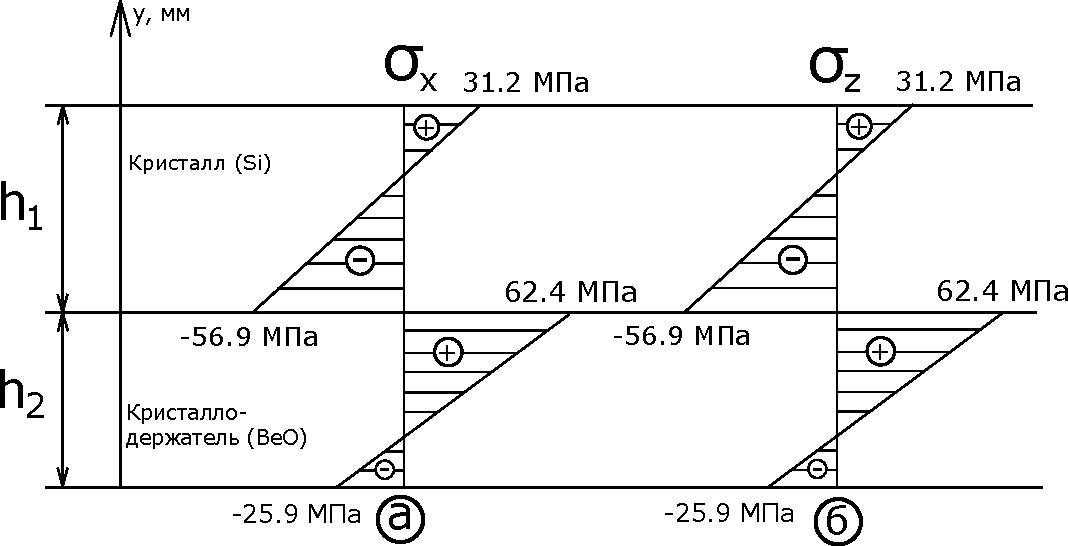
\includegraphics[width=0.8\linewidth]{epure.pdf}
    \caption{Эпюры распределения напряжений по толщине сборки: а "--- по короткой стороне, б "--- по длинной стороне}
    \label{fig:epure}
\end{figure}

Анализ эпюр распределения напряжений по толщине сборки показывает, что кристалл кремния испытывает небольшое растяжение на свободной поверхности и сжатие на границе раздела с кристаллодержателем. Кристаллодержатель на границе раздела с кристаллом испытывает растяжение, а на свободной поверхности "--- сжатие.

Максимальное напряжение в слое кристалла возникает по осям $x$ и $z$ на границе раздела с кристаллодержателем $|\sigma_{\max \text{ \BPChem{Si}}}| = 56.9 \text{ } МПа$.
Допускаемое напряжение для материала кристалла (\BPChem{Si}) определяется по формуле
\[
    [\sigma]_\text{\BPChem{Si}} = \frac{\sigma_\text{в \BPChem{Si}}}{n} = \frac{700}{2} = 350 \text{ } МПа.
\]

Условие прочности выполняется, так как
\[
    |\sigma_{\max \text{ \BPChem{Si}}}| = 56.9 \text{ } МПа < [\sigma]_\text{\BPChem{Si}} = 350 \text{ } МПа.
\]

Максимальное напряжение в слое кристаллодержателя возникает по осям $x$ и $z$ на границе раздела с кристаллом $|\sigma_{\max \text{ \BPChem{BeO}}}| = 62.4 \text{ } МПа$.
Допускаемое напряжение для материала кристаллодержателя (\BPChem{BeO}) определяется по формуле
\[
    [\sigma]_\text{\BPChem{BeO}} = \frac{\sigma_\text{в \BPChem{BeO}}}{n} = \frac{1900}{2} = 950 \text{ } МПа.
\]

Условие прочности выполняется, так как
\[
    |\sigma_{\max \text{ \BPChem{BeO}}}| = 62.4 \text{ } МПа < [\sigma]_\text{\BPChem{BeO}} = 950 \text{ } МПа.
\]

Так как обеспечивается прочность слоёв кристалла и кристаллодержателя, то обеспечивается прочность всей сборки в целом.
